% Section 2.2: The Astrophysical Gamma-Ray Sky
% Structure: Introduction -> Galactic Sources -> Extragalactic Sources

\section{Astrophysical Gamma-Ray Sources}
\label{sec:astro_sky}

The high-energy sky observed by the Fermi Large Area Telescope (Fermi-LAT) is a complex superposition of processes spanning our local Galactic neighborhood and the broader universe.
Phenomenologically, this emission falls into two domains.
The Galactic sky is dominated by the diffuse foreground of cosmic-ray interactions and populated by Galactic gamma-ray sources, most notably pulsars.
The extragalactic sky, in contrast, is characterized by an isotropic background arising primarily from unresolved \glspl{AGN_} and \glspl{SFG_}.
A detailed understanding of the astrophysical processes behind these conventional emitters is necessary for dark matter indirect detection, where every ordinary astrophysical signal is a potential background.

\subsection{Galactic Sources}
\label{sec:galactic_sources}

The gamma-ray emission from the Milky Way comprises two broad components: a diffuse foreground and a diverse population of individual point sources.
The \GDE dominates the observed sky and, as discussed in Section~\ref{sec:gde_model}, its template-based modeling remains the largest source of systematic uncertainty in Fermi-LAT analyses.
Alongside this diffuse foreground, the Galactic sky is populated by individual energetic sources, among which pulsars are the most prominent gamma-ray emitters.

Young pulsars are rapidly spinning neutron stars with large surface magnetic fields ($10^{11}$--$10^{13}$~G), emitting gamma rays primarily through curvature radiation in their magnetospheric gaps.
This emission typically continues over millions of years as the pulsar gradually decelerates (spins down).
Over longer timescales, neutron stars in binary systems can undergo a recycling process: the older neutron star accretes matter and angular momentum from its companion, spinning back up to periods of 2--10 milliseconds \cite{1982Natur.300..728A}.
These \glspl{MSP_} possess weaker magnetic fields ($10^8$--$10^9$~G) but maintain their rapid rotation for gigayears.
While young pulsars remain tightly clustered near their birthplaces in the Galactic disk, \glspl{MSP_} have orbited the Galaxy numerous times.
Their natal kicks and prolonged dynamical history broaden their spatial distribution, causing \gls{MSP_} populations to extend to higher Galactic latitudes and to densely populate the Galactic bulge \cite{Calore:2014oga}.

Their concentration in the Galactic bulge places \glspl{MSP_} squarely in the regions most targeted by dark matter searches, but the challenge extends beyond spatial overlap: curvature radiation produces a characteristic power-law spectrum with an exponential cutoff at a few GeV.
This spectral shape is basically indistinguishable from the expected photon yield of a $\sim$50~GeV \gls{WIMP_} annihilating into $b\bar{b}$ quarks \cite{Cirelli:2024ssz} --- a topic we will extensively explore in Chapters~\ref{ch:4} and \ref{ch:5}.

% MSPs detected in the Galactic plane have mean luminosities of $\langle L_\gamma \rangle \sim 10^{33}$--$10^{34}$~erg/s \cite{Hooper:2015jlu}, but the population closer to the Galactic center may differ in age, metallicity, and binary history.
% Breaking the spectral degeneracy between WIMP annihilation and unresolved MSPs therefore requires independent constraints on this luminosity function.
% One effective approach is to measure it in relatively clean environments with known distances, such as globular clusters.
% These dense stellar environments act as efficient factories for the binary systems necessary for MSP recycling.
% By characterizing the luminosity function of globular cluster MSPs, one can derive constraints that can be extrapolated to the broader Galactic bulge population.
% This is the approach adopted in Chapter~4, where we use simulation-based inference to measure the MSP luminosity function and scrutinize the origin of the GCE.

Among the remaining Galactic gamma-ray sources, \glspl{SNR_} and pulsar wind nebulae are routinely detected by the Fermi-LAT but represent subdominant backgrounds for the \blue{GeV} dark matter searches undertaken in this thesis.
\blue{On the other hand, at TeV energies, pulsar wind nebulae and \glspl{SNR_} are among the brightest sources in the sky, and they become a significant background for searches targeting the Galactic Center and the Galactic plane with instruments like \gls{CTAO_}. Extragalactic analyses at high Galactic latitude, such as the cross-correlation study of Chapter~\ref{ch:8}, instead evade these populations by masking the Galactic plane and the resolved sources.}

% Having surveyed the Galactic foreground and its point-source populations, we now turn to the extragalactic sky.

% \begin{figure}[t]
% 	\centering
% 	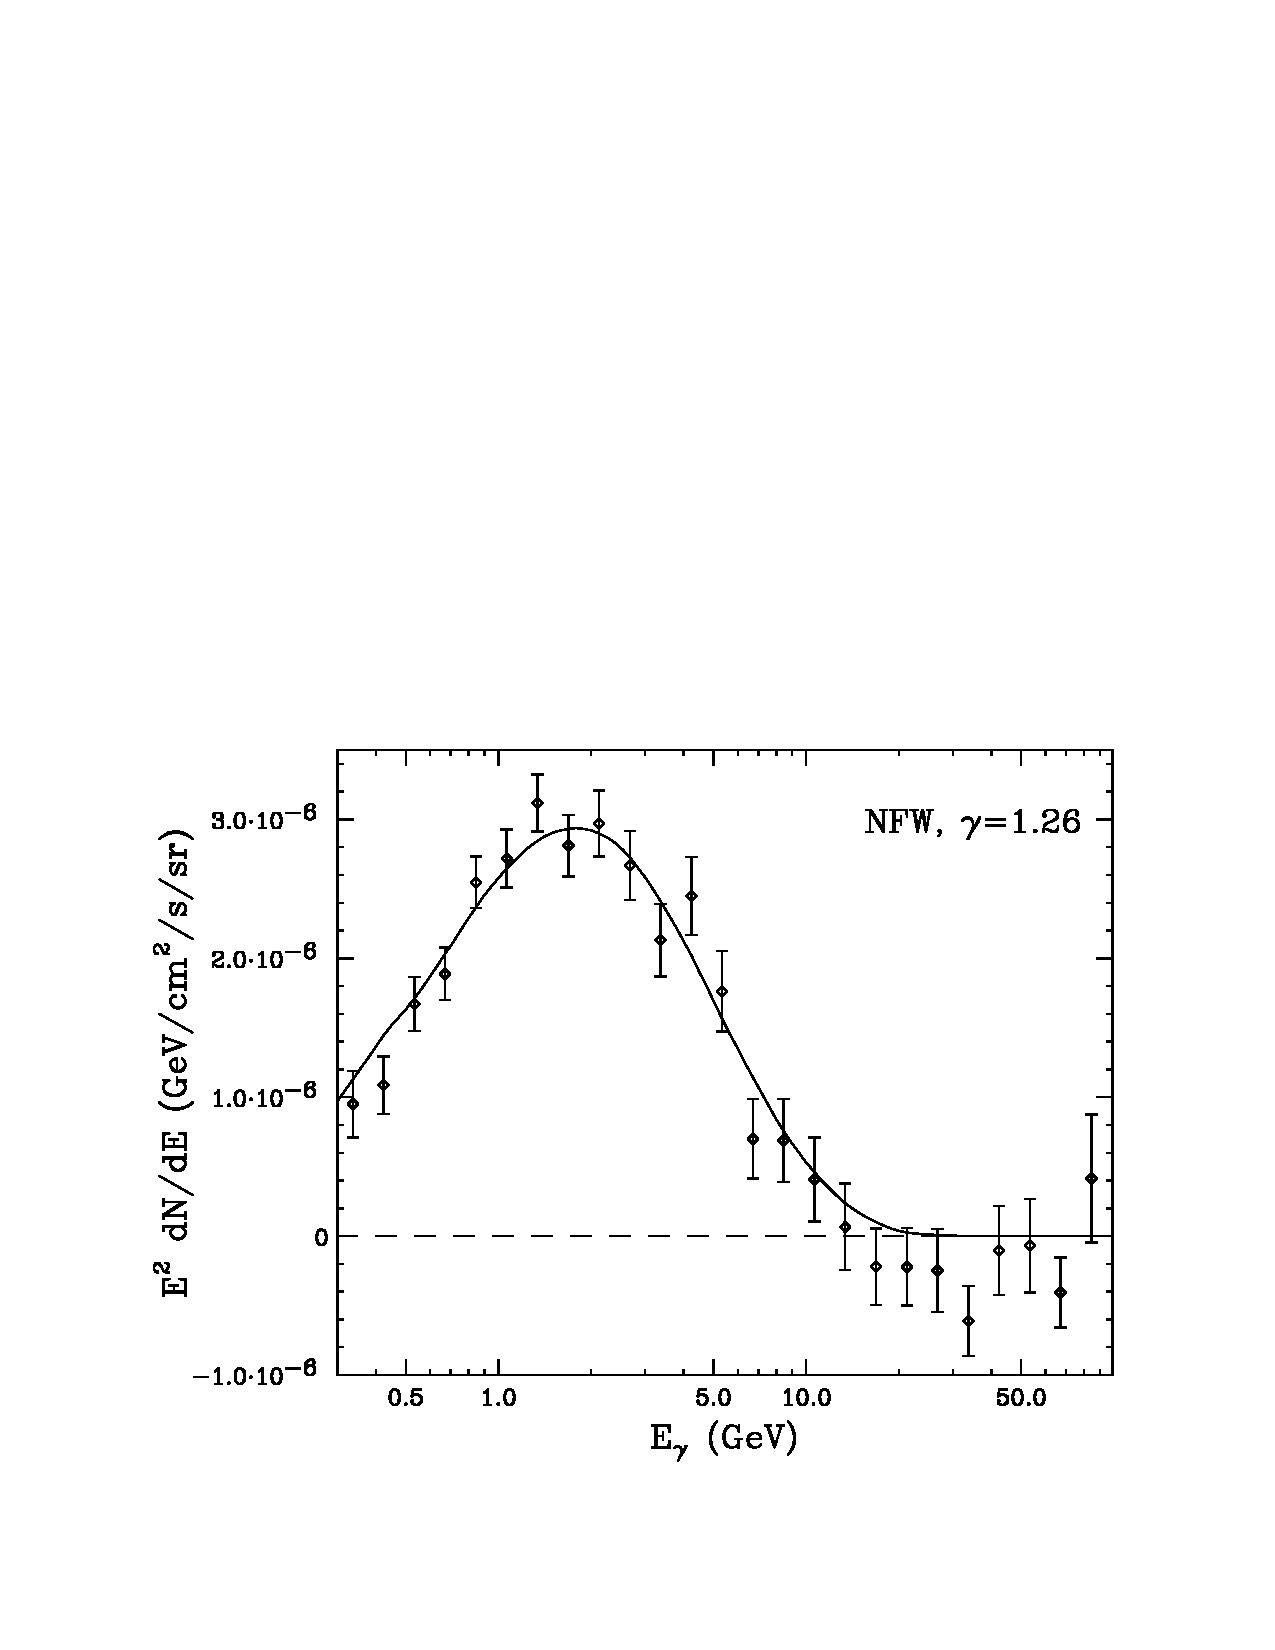
\includegraphics[width=0.7\columnwidth]{figures/gce_spectrum.pdf}
% 	\caption{The energy spectrum of the Galactic Center GeV excess fitted with a dark matter annihilation model ($b\bar{b}$ channel, $\sim$45 GeV).
% 		This spectral shape is highly degenerate with the curvature radiation spectrum of a population of millisecond pulsars.
% 		Credit: Figure 9.2 from Cirelli et al.\ (2024) \cite{Cirelli:2024ssz}.
% 	}
% 	\label{fig:gce_spectrum}
% \end{figure}

\subsection{Extragalactic Sources}
\label{sec:extragalactic_sources}

The high-latitude sky is dominated by the \gls{EGB_}, which encompasses the total gamma-ray emission originating outside our Galaxy.
The \EGB combines both individually resolved extragalactic sources and the unresolved glow of fainter objects \cite{DGRB-review,Ajello:2015mfa}.
The \gls{UGRB_} is the residual, almost isotropic emission that remains after subtracting the \GDE and all cataloged point sources \cite{Fermi-LAT:2014ryh,DGRB-review}. It is composed by the cummulative emission of all the currently unresolved gamma-ray sources, plus a residual truly diffuse isotropic background.
The Fermi-LAT has measured the \UGRB from 100~MeV to 820~GeV, and characterizing its composition is essential for identifying the origins of high-energy cosmic radiation and for constraining dark matter annihilation.

The dominant contributors to the extragalactic sky are blazars, a subclass of \glspl{AGN_} with relativistic jets oriented along the observer's line of sight.
Accretion onto a supermassive black hole powers these jets, producing a bimodal \gls{SED_} with a low-frequency synchrotron peak and a high-frequency inverse-Compton peak \cite{DGRB-review}.
Blazars are classified into two populations: \glspl{FSRQ_} and BL Lacertae objects (BL Lacs).
\Glspl{FSRQ_} exhibit broad optical emission lines and typically have lower-frequency synchrotron peaks, resulting in softer gamma-ray spectra that contribute most to the background below 1~GeV.
BL Lacs lack strong emission lines, have harder energy spectra, and frequently exhibit high-frequency synchrotron peaks.
As a result, nearby, low-luminosity BL Lacs produce the majority of the \EGB emission above 100~GeV \cite{Ajello:2015mfa}.
At these energies, gamma rays interact with the \gls{EBL_} to produce electron-positron pairs, an attenuation effect that naturally explains the exponential cutoff observed in the \EGB spectrum above roughly 250~GeV.
As a unified class, resolved and unresolved blazars account for approximately $50^{+12}_{-11}$\% of the total \EGB photons \cite{Ajello:2015mfa}.
Because they define both the resolved catalogs and the upper end of the unresolved background, the classification and modeling of blazars are central to the research presented in Chapters~\ref{ch:5}, \ref{ch:6}, and~\ref{ch:7}.

The remainder of the extragalactic gamma-ray emission is primarily due to \glspl{mAGN_} and \glspl{SFG_}.
\Glspl{mAGN_}, including Fanaroff-Riley radio galaxies, possess jets oriented away from our line of sight \cite{DGRB-review}.
Without strong Doppler boosting, they are intrinsically fainter than blazars but far more abundant, contributing an estimated 20\% to 25\% of the \UGRB \cite{DGRB-review,DiMauro:2013xta}.
\Glspl{SFG_}, on the other hand, produce gamma rays through hadronic interactions as described in Section~\ref{sec:hadronic}: cosmic-ray protons accelerated by supernovae collide with interstellar gas to produce neutral pions that decay into gamma rays.
While their individual luminosities are low, \glspl{SFG_} are ubiquitous and their aggregate emission closely tracks the cosmic star-formation history.
Current models suggest they account for 10\% to 30\% of the \EGB \cite{Ajello:2015mfa,Tamborra:2014xia}, potentially dominating among the faintest source populations.

\blue{Beyond these steady populations, the extragalactic sky is punctuated by transient sources.
Gamma-ray bursts --- the prompt, seconds-long flashes accompanying stellar collapse or compact-object mergers --- and week-long blazar flares can briefly outshine every steady source in the sky.
They play a marginal role as backgrounds for the population studies of this thesis, but they are physics targets in their own right.
The spectra of bright flaring sources and the gamma-ray counterparts of core-collapse supernovae have been used to search for axion-like particles converting to photons in astrophysical magnetic fields~\cite{Fermi-LAT:2016nkz,Payez:2014xsa} (cf.\ Section~\ref{sec:targets}).}

Detailed population models demonstrate that the combined emission from blazars, \glspl{mAGN_}, and \glspl{SFG_} can account for the entire amplitude and spectral shape of the measured \EGB (Figure~\ref{fig:egb_composition}), establishing tight constraints on any dark matter contribution \cite{Ajello:2015mfa}.

The connection between resolved source catalogs and the unresolved background \blue{is made quantitative by} the source-count distribution, $dN/dS$, which describes the differential number density of sources per unit solid angle as a function of their gamma-ray flux $S$.
Integrating the $dN/dS$ distribution from zero flux up to the telescope's point-source detection threshold yields the intensity of the \UGRB.
While the bright end of the $dN/dS$ is directly anchored by catalog measurements, probing the distribution below the detection threshold requires statistical techniques that extract population-level information from the collective imprint of unresolved sources on the photon-count map.
The formal definition of $dN/dS$, its connection to the underlying luminosity function, and the methods developed to reconstruct it in the unresolved regime are the subject of Chapter~\ref{ch:6}.

\begin{figure}[t]
	\centering
	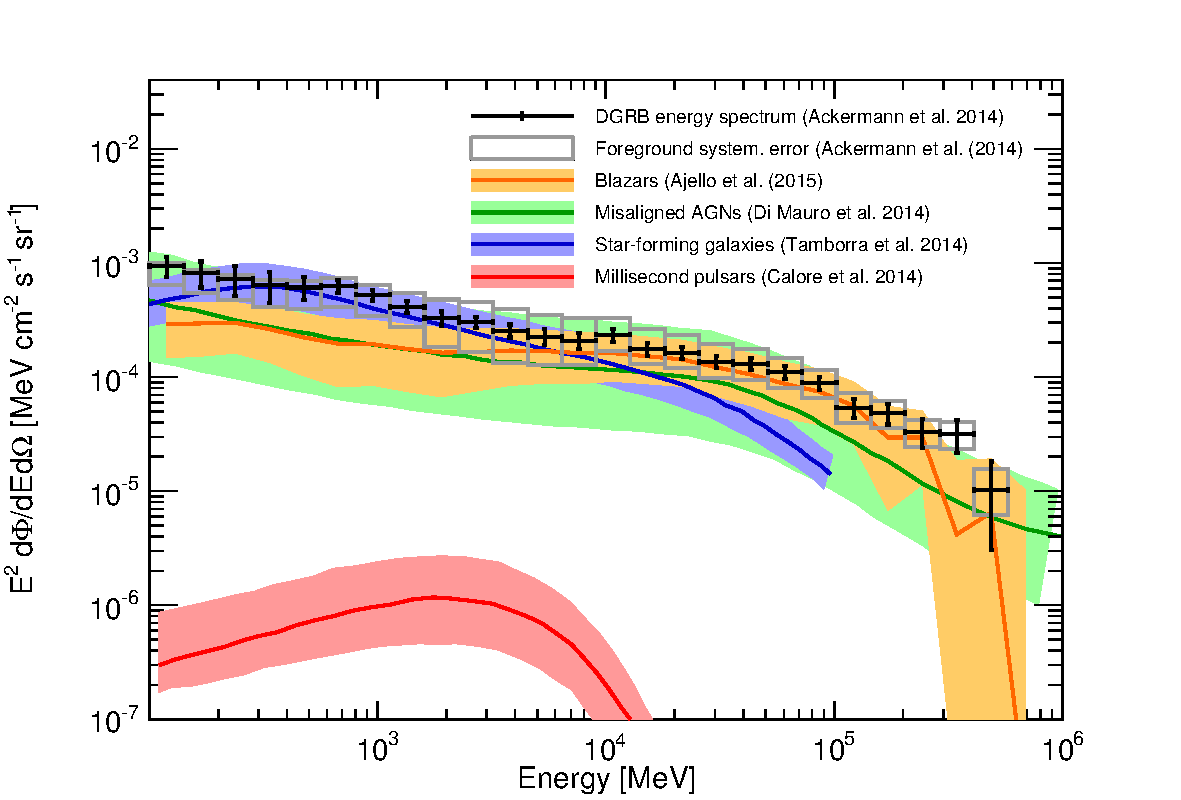
\includegraphics[width=0.7\columnwidth]{chapter_02/figures/egb_composition.pdf}
	\caption{The energy spectrum of the \gls{DGRB_} and its expected composition.
		The black points represent the Fermi-LAT measurement, with gray bands indicating systematic uncertainty from the Galactic diffuse foreground subtraction.
		The colored lines and bands illustrate the predicted contributions from unresolved blazars (orange), \glspl{mAGN_} (green), \glspl{SFG_} (blue), and \glspl{MSP_} (red).
		Credit: Figure 9 from \cite{DGRB-review}.
	}
	\label{fig:egb_composition}
\end{figure}
